% 2006 年全国卷Ⅰ文科第 20 题：互相垂直的异面直线
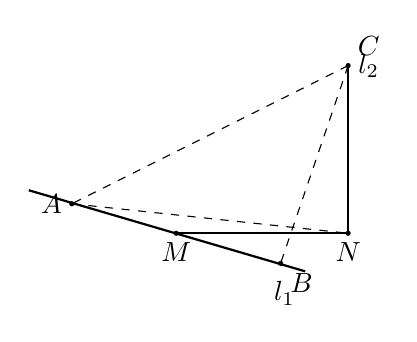
\begin{tikzpicture}[>=stealth,scale=0.78]
  \coordinate (A) at (0.55,1.20);
  \coordinate (M) at (2.25,0.72);
  \coordinate (B) at (3.95,0.23);
  \coordinate (N) at (5.05,0.72);
  \coordinate (C) at (5.05,3.45);
  \draw[thick] (-0.15,1.42)--(4.35,0.10) node[below left] {$l_1$};
  \draw[thick] (N)--(C) node[right] {$l_2$};
  \draw[thick] (M)--(N);
  \draw[dashed] (A)--(N) (C)--(A) (C)--(B);
  \fill (A) circle (1.2pt) node[left] {$A$};
  \fill (M) circle (1.2pt) node[below] {$M$};
  \fill (N) circle (1.2pt) node[below] {$N$};
  \fill (B) circle (1.2pt) node[below right] {$B$};
  \fill (C) circle (1.2pt) node[above right] {$C$};
\end{tikzpicture}
